\part{IHM}
\setcounter{section}{0}

\section{Enchainement des fenêtres - EDF}

\begin{figure}[H]
\noindent\makebox[\textwidth]{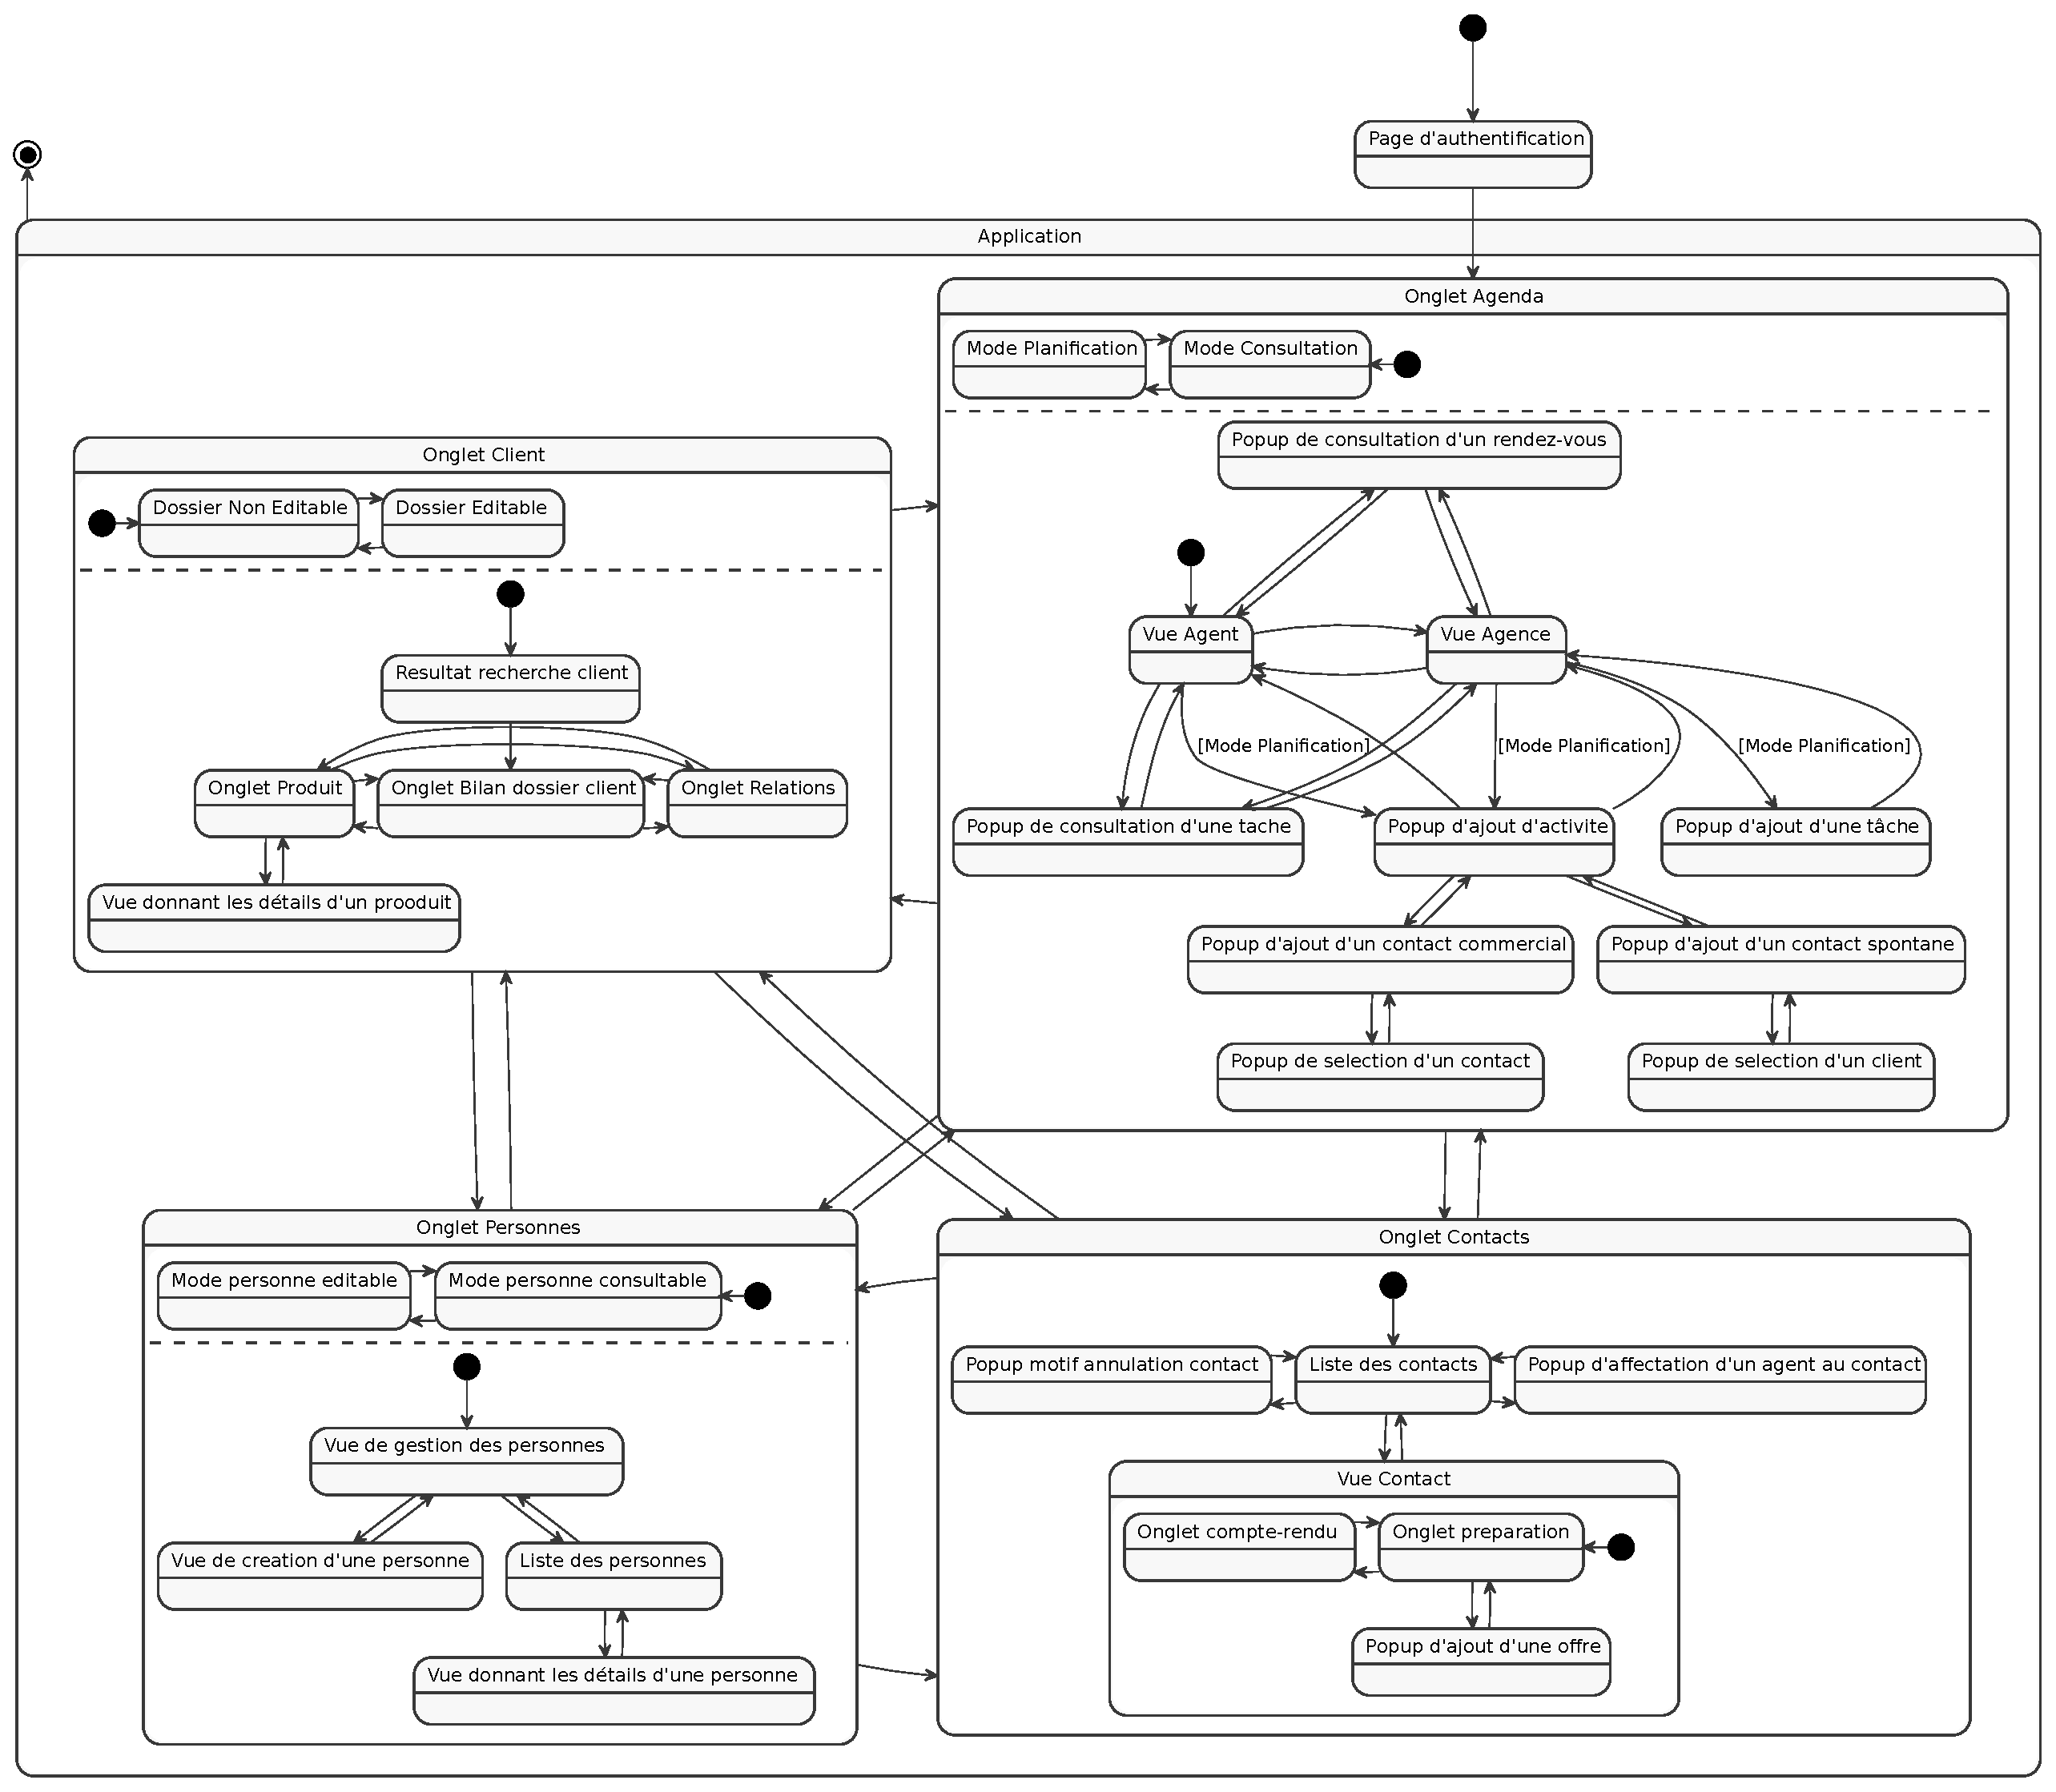
\includegraphics[width=18cm]{figures/eps/EdF}}
\caption{Diagramme d'enchainement des fenêtres}
\end{figure}

\section{Présentation des différentes vues}
Les vues de l'IHM sont présentées dans les pages suivantes. Les différents services appelés sont indiqués à côté de celles-ci.


\includepdf[scale=0.8,angle=90,pages={2-9},pagecommand=\subsection{IHM client}]{figures/IHM.pdf}


\begin{table}[H]
\centering
\caption{SMA - IHM Client (ref 1)}
\begin{tabular}{lll}
\hline
Num & \multicolumn{1}{c}{Nom Contrôle} & \multicolumn{1}{c}{SMA} \\ \hline
\rowcolor[gray]{0.9}
\multicolumn{3}{l}{CU10 - Recherche des clients}  \\
1.1 & Bouton Rechercher & PAS DE SMA \\
\rowcolor[gray]{0.9}
\multicolumn{3}{l}{CU10 - Résultats recherche clients} \\ 
1.2 & Bouton Rechercher  & PAS DE SMA       \\             
1.3 & Bouton Voir le client & PAS DE SMA \\
\multicolumn{3}{l}{CU10 - Recherche des clients}  \\
1.1 & Bouton Rechercher & PAS DE SMA \\
\rowcolor[gray]{0.9}
\multicolumn{3}{l}{CU10 - Résultats recherche clients} \\ 
1.2 & Bouton Rechercher  & PAS DE SMA       \\             
1.3 & Bouton Voir le client & PAS DE SMA \\
\rowcolor[gray]{0.9}
\multicolumn{3}{l}{CU10 - Recherche des clients}  \\
1.1 & Bouton Rechercher & PAS DE SMA \\
\rowcolor[gray]{0.9}
\multicolumn{3}{l}{CU10 - Résultats recherche clients} \\ 
1.2 & Bouton Rechercher  & PAS DE SMA       \\             
1.3 & Bouton Voir le client & PAS DE SMA \\
1.2 & Bouton Rechercher  & PAS DE SMA       \\             
1.3 & Bouton Voir le client & PAS DE SMA \\
1.2 & Bouton Rechercher  & PAS DE SMA       \\             
1.3 & Bouton Voir le client & PAS DE SMA \\
\end{tabular}
\end{table}


\includepdf[scale=0.8,angle=90,pages={10-14},pagecommand=\subsection{IHM Personnes}]{figures/IHM.pdf}

\begin{table}[H]
\centering
\caption{SMA - IHM Personnes}
\label{my-label}
\begin{tabular}{ll}
\hline
\multicolumn{1}{c}{Num Contrôle} & \multicolumn{1}{c}{SMA} \\ \hline
\multicolumn{2}{c}{CU2 - Affectation contact}              \\
                                 &                         \\
                                 &                         \\ \hline
\end{tabular}
\end{table}


\includepdf[scale=0.8,angle=90,pages={15-25},pagecommand=\subsection{IHM Agenda}]{figures/IHM.pdf}

\begin{table}[H]
\centering
\caption{SMA - IHM Agenda}
\label{my-label}
\begin{tabular}{ll}
\hline
\multicolumn{1}{c}{Num Contrôle} & \multicolumn{1}{c}{SMA} \\ \hline
\multicolumn{2}{c}{CU2 - Affectation contact}              \\
                                 &                         \\
                                 &                         \\ \hline
\end{tabular}
\end{table}

\includepdf[scale=0.8,angle=90,pages={26-34},pagecommand=\subsection{IHM Contact}]{figures/IHM.pdf}

\begin{table}[H]
\centering
\caption{SMA - IHM Contact}
\label{my-label}
\begin{tabular}{ll}
\hline
\multicolumn{1}{c}{Num Contrôle} & \multicolumn{1}{c}{SMA} \\ \hline
\multicolumn{2}{c}{CU2 - Affectation contact}              \\
                                 &                         \\
                                 &                         \\ \hline
\end{tabular}
\end{table}